\documentclass[letterpaper]{article}
\usepackage[submission]{aaai2027}
\usepackage[hyphens]{url}
\usepackage{graphicx}
\urlstyle{rm}
\def\UrlFont{\rm}
\usepackage{natbib}
\usepackage{caption}
\frenchspacing
\setlength{\pdfpagewidth}{8.5in}
\setlength{\pdfpageheight}{11in}
\usepackage{booktabs}
\usepackage{amsmath}
\usepackage{multirow}
\pdfinfo{/TemplateVersion (2027.1)}
\setcounter{secnumdepth}{0}
\renewcommand{\thetable}{S\arabic{table}}
\renewcommand{\thefigure}{S\arabic{figure}}

\title{Supplementary Document\\
\large Use LLMs to Build Repair Tools, Not Patch Generation:\\Cost-Effective
Automated Program Repair}
\author{Anonymous submission}
\affiliations{}

\begin{document}
\maketitle

\noindent This document carries what the main paper's page budget could not.
Nothing here introduces a claim the paper does not already make: each item is
the tabular or graphical form of a number the Results section gives, or a
measurement the paper cites without room to print. Assignment ids (R1--R5,
C1--C6), the arm names, and every metric definition are the main paper's.
Values are generated from \texttt{results/} by the released scripts
(\texttt{run.py tables}, \texttt{run.py figures}, \texttt{run.py labelagree});
none is transcribed.

\section{What Escalation Costs, Assignment by Assignment}

Table~\ref{tab:cost} gives the escalation rate $e$ per assignment, the calls it
buys, the local search time, and the one-off build. The rate is what the cost
argument turns on: an assignment that escalates rarely is one whose frozen tool
is carrying the class on its own, and the two assignments above 20\% are the
two where the reference pool is thinnest relative to the variety of the
submissions.

\begin{table}[h]
\centering\small\setlength{\tabcolsep}{4pt}
\begin{tabular}{lrrrr}
\toprule
& $e$ (\%) & calls & $\mathrm{ATT}_{\mathrm{cpu}}$ (s) & build (min) \\
\midrule
R1 & 0.7 & 8 & 2.28 & 32 \\
R2 & 22.5 & 196 & 3.18 & 27 \\
R3 & 0.0 & 0 & 1.83 & 18 \\
R4 & 9.2 & 66 & 3.43 & 28 \\
R5 & 0.9 & 2 & 4.79 & 18 \\
C1 & 13.2 & 116 & 3.17 & 20 \\
C2 & 23.3 & 261 & 2.22 & 38 \\
C3 & 13.0 & 18 & 6.94 & 3 \\
C4 & 5.3 & 4 & 1.34 & 12 \\
C5 & 15.6 & 24 & 4.86 & 4 \\
C6 & 66.7 & 4 & 6.58 & 6 \\
\midrule
\textbf{All} & \textbf{11.8} & \textbf{699} & \textbf{2.88} & \textbf{206} \\
\bottomrule
\end{tabular}

\caption{Escalation and cost per assignment, \texttt{claude-sonnet-5}.}
\label{tab:cost}
\end{table}

\section{Robustness}

Table~\ref{tab:robust} puts three axes side by side: assignment difficulty, the
choice of builder, and the escalation threshold. The difficulty bands group the
eleven assignments as CS1, Codeforces 800--1000, and Codeforces 1200--2000, the
last folding C6's three submissions in rather than reporting them alone.

\begin{table}[h]
\centering\scriptsize\setlength{\tabcolsep}{1pt}
\resizebox{\columnwidth}{!}{\begin{tabular}{@{}l@{\hskip 4pt}ccc@{}}
\toprule
& Refactory & PyDex & \textsc{CoEP}\textsubscript{LF} \\
Stratum & \multicolumn{3}{c}{RR (\%) / RPS} \\
\midrule
\multicolumn{4}{l}{\emph{Difficulty} (\texttt{claude-sonnet-5})}\\
\quad CS1 & 90.8 / 0.397 & 98.6 / 0.382 & 99.4 / 0.279 \\
\quad CF 800--1000 & 83.1 / 0.663 & 99.4 / 0.942 & 100.0 / 0.572 \\
\quad CF 1200--2000 & 54.5 / 0.815 & 100.0 / 0.800 & 100.0 / 0.693 \\
\midrule
\multicolumn{4}{l}{\emph{Builder}}\\
\quad \texttt{claude-sonnet-5} & -- & 99.0 / 0.598 & 99.7 / 0.404 \\
\quad \texttt{gpt-5.4-mini} & -- & 98.9 / 0.669 & 99.7 / 0.417 \\
\midrule
\multicolumn{4}{l}{\emph{Threshold}, 29 measured settings}\\
\quad range & -- & -- & 99.7 / 0.378--0.451 \\
\quad spend & \multicolumn{3}{c}{\$12.47--\$15.61 total} \\
\bottomrule
\end{tabular}
}
\caption{Difficulty, builder, and escalation threshold.}
\label{tab:robust}
\end{table}

Figure~\ref{fig:gate} plots every measured threshold setting against the
baselines it is compared to. The point is the emptiness between the cluster and
the baselines: the whole family spans \$12.47--\$15.61 of total spend, so which
setting ships cannot change a conclusion. The shipped rule, escalate a passing
local patch whose $\mathrm{RPS}$ exceeds 1, is marked with a star and is the
canonical run rather than the sweep's reconstruction of it.

\begin{figure}[h]
\centering
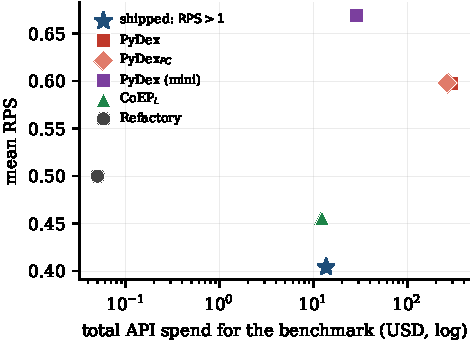
\includegraphics[width=\columnwidth]{../figures/fig_gate.pdf}
\caption{Mean RPS against total spend. Each small marker is one threshold
setting; the star is the shipped rule. Repair rate is identical across all of
them.}
\label{fig:gate}
\end{figure}

\section{Do the Rule Names Say What the Rules Do?}

The paper claims an auditable name for every repair its rules make, and this is
the measurement behind that claim. Three raters independently judged all
\textbf{195} rules the two builders wrote, each against the rule's own source
and one repair it actually produced, preferring a repair no other rule
contributed to so the edit is attributable. Four rules the rating guide had
worked through as examples are excluded, leaving \textbf{191}.

The scheme has three values, applied in a fixed order so that the two questions
do not blur. A name is \texttt{wrong} if it contradicts the rule's main
behaviour; otherwise \texttt{accurate} if it identifies a misconception, and
\texttt{describes\_edit} if it states the edit correctly without saying what
the student misunderstood. Only the first of these bears on the paper's claim;
the second distinction is reported here for completeness.

\begin{table}[h]
\centering\small\setlength{\tabcolsep}{5pt}
% Static: this track's supplement is not a target of `run.py tables`.
% Regenerate with `run.py labelagree`.
\begin{tabular}{lrrr}
\toprule
& accurate & describes\_edit & wrong \\
\midrule
Rater 1 & 46.6 & 45.5 & 7.9 \\
Rater 2 & 47.6 & 42.9 & 9.4 \\
Rater 3 & 50.3 & 42.4 & 7.3 \\
\midrule
Majority, per rule & 47.1 & 44.5 & \textbf{8.4} \\
Majority, per repair & 37.3 & 62.0 & \textbf{0.7} \\
\bottomrule
\end{tabular}
\caption{Rule-name labelling, in per cent. Per-rule rows count the 191 rules;
the per-repair row weights each rule by the repairs it produced, which is the
side a student sees.}
\label{tab:labels}
\end{table}

Agreement is Fleiss' $\kappa = 0.890$ over three raters and three categories,
with all three agreeing on 173 of the 191 rules (90.6\%); pairwise raw
agreement is 94.8\%, 93.2\% and 93.2\%. The per-rater marginals in
Table~\ref{tab:labels} are close enough that no rater is driving the result.

Two asymmetries are worth stating. All \textbf{16} names judged \texttt{wrong}
were written by \texttt{gpt-5.4-mini}; \texttt{claude-sonnet-5} wrote none, and
\textbf{14} of the 16 never fire, which is why a rate of 8.4\% of rules is
0.7\% of repairs. And 66 of the 195 rules never produced a repair, so the
per-rule and per-repair rows answer different questions: the first is what the
builder wrote, the second is what a class would actually see.

\section{What the Builder Writes}

Table~\ref{tab:rules} lists the rules that carry the most submissions, counted
as distinct submissions rather than as applications, since a repair may compose
several rules. The distinction that matters is reuse: of the 128 rules the
builders wrote and that fired, exactly one fired on more than one assignment,
\texttt{add\_missing\_call\_parens}, which describes a Python trap rather than
anything about a problem. The always-on rules recur everywhere by construction,
which is why the builder's layer is priced per assignment and they are not.

\begin{table}[h]
\centering\scriptsize\setlength{\tabcolsep}{3pt}
\resizebox{\columnwidth}{!}{\begin{tabular}{llrr}
\toprule
Rule & where & submissions & assignments \\
\midrule
\texttt{generic\_flip\_compare} & always-on & 263 & 10 \\
\texttt{append\_missing\_return\_len\_after\_loop} & R1 & 114 & 1 \\
\texttt{slice\_case\_check\_to\_equality} & C2 & 108 & 1 \\
\texttt{generic\_shift\_index} & always-on & 74 & 5 \\
\texttt{strict\_one\_should\_be\_exactly\_one} & R2 & 70 & 1 \\
\texttt{count\_compare\_relax} & R2 & 58 & 1 \\
\texttt{generic\_shift\_range} & always-on & 50 & 7 \\
\texttt{capitalize\_title\_to\_swapcase} & C2 & 43 & 1 \\
\midrule
\multicolumn{4}{l}{128 builder-written rules fired, 1 on more than one assignment} \\
\bottomrule
\end{tabular}
}
\caption{The eight rules repairing the most submissions.}
\label{tab:rules}
\end{table}

\section{Self-Learning}

\begingroup\sloppy
The eight rules self-learning absorbed read as misconceptions in the same way.
On R2 with \texttt{claude-sonnet-5}: \texttt{counter\_var\_confusion},
\texttt{uniqueness\_\allowbreak count\_gt1\_to\_neq1},
\texttt{index\_vs\_count\_\allowbreak and\_uncalled\_bool},
\texttt{missing\_else\_false}. On R2 with \texttt{gpt-5.4-mini}:
\texttt{count\_equality\_for\_uniqueness},
\texttt{count\_uniqueness\_\allowbreak instead\_of\_\allowbreak direct\_membership},
\texttt{missing\_call\_\allowbreak and\_predicate\_fix}. On C3:
\texttt{binarysearch\_zero\_exit}.
\endgroup

\section{Reproducibility}

The repository contains the harness, every prompt, the 22 synthesized
repairers with their build costs, the per-submission event log each arm wrote,
and the rating sheet with all three raters' returned labels. Five commands
regenerate every number in both documents from those logs without touching a
model: \texttt{run.py tables}, \texttt{run.py figures}, \texttt{run.py
numbers}, which recomputes each quantity and reports whether the string still
occurs in the paper, \texttt{run.py stats}, and \texttt{run.py labelagree}.
The measured threshold settings are archived as
\texttt{results/threshold\_sweep.json}, and the labelling sheet, its guide and
the three returned files as \texttt{results/rules*.csv} and
\texttt{results/labeling\_guide.md}.

Two dependencies are outside our control and worth stating. Both builders are
closed commodity models reached through their providers' APIs, so a rebuild
cannot be guaranteed to reproduce the same rules; what is released is the tools
those builds produced, which are ordinary Python and run offline. Refactory's
replication package is its authors' and is cloned rather than vendored.

\end{document}
